\documentclass[tikz,border=4pt]{standalone}
\usepackage{pgfplots}
\pgfplotsset{compat=1.18}
\usepgfplotslibrary{fillbetween}
\usetikzlibrary{arrows.meta,positioning,calc,shapes.geometric}
\begin{document}
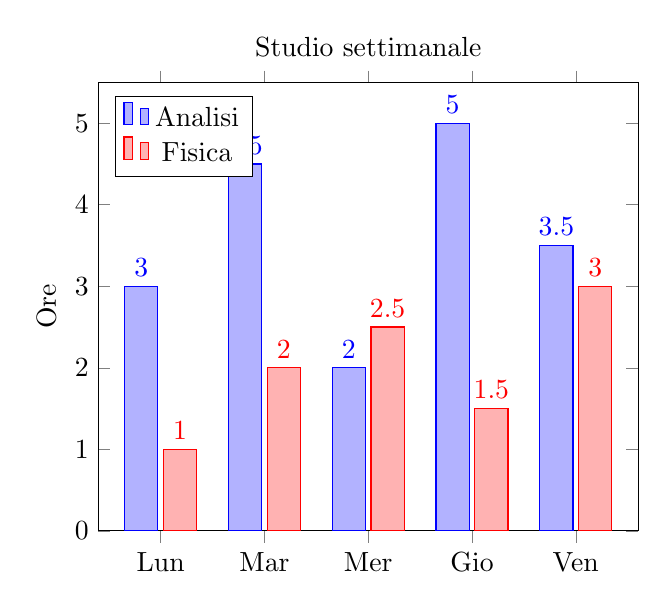
\begin{tikzpicture}
  \begin{axis}[
      ybar, bar width=12pt, ymin=0,
      symbolic x coords={Lun,Mar,Mer,Gio,Ven}, xtick=data,
      ylabel={Ore}, title={Studio settimanale},
      nodes near coords, enlarge x limits=0.15,
      legend pos=north west]
    \addplot coordinates {(Lun,3) (Mar,4.5) (Mer,2) (Gio,5) (Ven,3.5)};
    \addplot coordinates {(Lun,1) (Mar,2) (Mer,2.5) (Gio,1.5) (Ven,3)};
    \legend{Analisi, Fisica}
  \end{axis}
\end{tikzpicture}
\end{document}
